\documentclass{article}

% Boilerplate {{{

\usepackage{amsmath}
\usepackage{unicode-math}
\setmainfont{XITS}
\setmathfont{XITS Math}
\usepackage{tikz}
\usetikzlibrary{matrix}
\usepackage{newunicodechar}
\usepackage{galois}
\usepackage{amsthm}

\theoremstyle{definition}
\newtheorem*{definition}{Definition}
\newtheorem*{example}{Example}

\theoremstyle{plain}
\newtheorem*{lemma}{Lemma}
\newtheorem{theorem}{Theorem}
\newtheorem{corrolary}{Corrolary}

\newcommand{\iif}{\underline{\text{if}}}
\newcommand{\case}{\underline{\text{case}}}
\newcommand{\halt}{\underline{\text{halt}}}
\newcommand{\lam}{\underline{\text{λ}}}
\newcommand{\add}{\text{add1}}
\newcommand{\sub}{\text{sub1}}
\newcommand{\gez}{\text{gez}}
\newcommand{\INT}{\text{INT}}
\newcommand{\TRUE}{\text{TRUE}}
\newcommand{\FALSE}{\text{FALSE}}
\newcommand{\ddo}{\operatorname{do}}
\newcommand{\llet}{\operatorname{let}}
\newcommand{\return}{\operatorname{return}}
\newcommand{\getstore}{\operatorname{get-σ}}
\newcommand{\putstore}{\operatorname{put-σ}}
\newcommand{\getenv}{\operatorname{get-ρ}}
\newcommand{\putenv}{\operatorname{put-ρ}}
\newcommand{\gettime}{\operatorname{get-τ}}
\newcommand{\puttime}{\operatorname{put-τ}}
\newcommand{\coercebool}{\operatorname{↓𝔹}}
\newcommand{\coercekon}{\operatorname{↓λ₁}}
\newcommand{\coercefun}{\operatorname{↓λ₂}}
\newcommand{\liftpowerset}{\operatorname{↑𝒫}}
\newcommand{\touchedcall}{\operatorname{𝓉𝒞}}
\newcommand{\touchedvar}{\operatorname{𝓉Var}}

\newcommand{\C}{L}
\newcommand{\A}{\widehat{L}}

\newcommand{\Csteps}{↦}
\newcommand{\Asteps}{\ \widehat{↦}\ }

\newcommand{\Ce}{e}
\newcommand{\Ae}{\widehat{e}}

\newcommand{\AStore}{\widehat{Store}}
\newcommand{\AEnv}{\widehat{Env}}
\newcommand{\ATime}{\widehat{Time}}
\newcommand{\AVal}{\widehat{Val}}

\newcommand{\PM}{𝒫\ }
\newcommand{\PT}{𝒫_T\ }

\newcommand{\SM}{State}
\newcommand{\ST}{State_T}

\newenvironment{donotbreak}
{\\[0.5\baselineskip]\begin{minipage}{\linewidth}}
{\end{minipage}\\[0.5\baselineskip]}

% \usepackage{multicol}

% \newunicodechar{λ}{\lambda}
% \newunicodechar{→}{\rightarrow}
% \newunicodechar{𝒯}{\mathcal{T}}
% \newunicodechar{∀}{\forall}
% \newunicodechar{∘}{\circ}
% \newunicodechar{𝒫}{𝒫\ }


% \usepackage{amssymb}
% \usepackage{listings}
% \usepackage{stmaryrd}
% \usepackage{wasysym}
% \usepackage{cite}
% \usepackage{pgfplots}
% \usepackage{minted}
% \usepackage{float}
% \usepackage{caption}
% \usepackage{fontspec}
% \setmonofont{Inconsolata}
% % \usepackage{hyperref}
% 
% \lstset{basicstyle=\footnotesize\ttfamily,language=haskell}
% \lstMakeShortInline|
% 
% \newmintedfile[haskell]{haskell}{}
% \newmintinline[h]{haskell}{}
% \newmintinline[p]{text}{}
% 
% \newenvironment{itemizenobreak}
% {\\[0.5\baselineskip]\begin{minipage}{\linewidth}\begin{itemize}}
% {\end{itemize}\end{minipage}\\[0.5\baselineskip]}
% 
% 
% \newcommand{\DSS}{\text{\lstinline|SS|}}
% \newcommand{\DSSAbs}{\widehat{\text{\lstinline|SS|}}}
% \newcommand{\Dstep}{\text{\lstinline|step|}}
% \newcommand{\DstepAbs}{\widehat{\text{\lstinline|step|}}}
% 
% %%% pulled from internet (stack overflow user Christian Feuersänger) %%%
% % argument #1: any options
% \newenvironment{customlegend}[1][]{%
%     \begingroup
%     % inits/clears the lists (which might be populated from previous
%     % axes):
%     \csname pgfplots@init@cleared@structures\endcsname
%     \pgfplotsset{#1}%
% }{%
%     % draws the legend:
%     \csname pgfplots@createlegend\endcsname
%     \endgroup
% }%
% 
% % makes \addlegendimage available (typically only available within an
% % axis environment):
% \def\addlegendimage{\csname pgfplots@addlegendimage\endcsname}
% 


\title{Abstract Control in Static Analysis (Draft)}
\author{David Darais}
\date{\today}

\begin{document}
\maketitle

% }}}

% Abstract {{{
\begin{abstract}

The field of static analysis offers many techniques for automatically discovering facts about programs.
For example, a static analysis might be used to verify that a program is memory safe, or that it obeys a privacy policy.
Techniques based on Abstract Interpretation (AI) allow the analysis designer to vary some properties of an analysis.
However, features like context, object, and flow sensitivity must be hard-coded into an analysis based on classic AI.
Abstracting Abstract Machines (AAM) is one design methodology for analysis which exposes more of these features as tuning knobs.
Unfortunately, AAM lacks reusable tools for building analyses, and not all analysis features fit nicely into the framework.

We propose a new compositional framework for designing analyses which supports a tuning knob missing from AAM: abstract control.
We achieve compositionality by refactoring AAM into monad transformers, each of which we relate back to abstract state machines.
When put together, these monad transformers build analyses which are correct by construction.
Furthermore, the monadic abstraction allows us to recover a tuning knob for abstract control when designing analyses.
Abstract control allows one to adjust the flow and path sensitivity of an analysis independent of other design choices.

\end{abstract}
% }}}

\tableofcontents

% Introduction {{{
\section{Introduction}
\label{section:Introduction}

Static analysis is useful for many different situations.
A software developer might use an analysis to find bugs in a program.
A software merchant might use an analysis to detect malware or other security vulnerabilities in software hosted by their app store.
A manufacturer might use an analysis to establish high assurance in the reliability of control software for a car or airplane.
Each of these situations requires a different type of analysis.
To meet the needs of a given problem, an analysis designer has two options: retrofit an existing analysis or design one from scratch.
Retrofitting an existing analysis can be insufficient because the tension between precision and performance is often too high.
Getting an analysis right might require more modification than an existing analysis was designed to support.
Because of this, complex analyses often need to be designed from scratch, and analysis designer need tools to help them with this process.

Designing a static analysis is hard.
Designing \emph{the right} static analysis is even more difficult.
One possible process for arriving at the right static analysis is:
\begin{enumerate}
\item Describe the semantics of your language.
\item Design an analysis which you hope has right properties.
\item Exercise the analysis.
\item If the analysis is too slow or imprecise: repeat from 2.
\end{enumerate}
To get a complex analysis right this process must be repeated multiple times.
Iterating quickly between the design and exercise of an analysis is the key to getting the analysis you wanted without too much pain.

One methodology which aims to ease the design process for static analysis is the Abstracting Abstract Machines (AAM) framework\cite{AAM}.
AAM separates two design steps which are traditionally tightly coupled: describing features of interest and abstracting those features.
Furthermore, AAM shows that the abstraction step is systematic, freeing the analysis designer to spend effort in designing features of interest.
However, AAM doesn't provide reusable tools for the design process; the analysis designer must describe their state machine transition from scratch.
Additionally, some analysis features like flow and path sensitivity don't fit nicely into the AAM framework.

We propose a new compositional framework for designing analyses which supports a tuning knob missing from AAM: abstract control.
To achieve this we refactor AAM into monad transformers.
Using monad transformers, the analysis designer can easily add and remove features from their semantics independently of other features.
The monadic abstraction additionaly exposes a new tuning knob for analyses which we call abstract control.
Abstract control allows one to adjust the flow and path sensitivity of an analysis independent of other design choices.

To justify the soundness of the approach, we show that the monad transformers we use are also galois connection transformers.
This means that any combination of our monad transformers will yield a sound approximation of a state machine semantics.

Our contributions in this work are:
\begin{enumerate}
\item A monadic formulation of AAM which exposes abstract control as a tuning knob.
\item A compositional analysis \emph{implementation} framework for building abstract state machines using monad transformers.
\item A compositional analysis \emph{proof} framework for justifying the correctness of abstract state machines using galois connection transformers.
\item A new monad transformer for nondeterminism which is the key to recovering abstract control as a tuning knob.
\end{enumerate}

The rest of the paper is structured as follows:
Section \ref{Background} covers necessary background material in semantics, analysis, and the CPS language which we use for examples.
Section \ref{MAAM} demonstrates a monadic variant of AAM which supports defining compositional interpreters for analysis.
Section \ref{AbstractControl} discusses abstract control and how we exploit the monadic abstraction to expose a tuning knob for it.
Section \ref{Optimizations} gives two examples of analysis optimizations and how they adapt seamlessly to variations in abstract control.
Section \ref{Correctness} discusses the correctness framework and what key lemmas are involved.
Section \ref{Proofs} shows proof steps in more detail for the arguments made in section \ref{Correctness}.
Sections \ref{RelatedWork} and \ref{FutureWork} discuss relate and future work, and section \ref{Conclusion} concludes.

% }}}

% Background {{{
\section{Background}
\label{section:Background}
% * Background
%   - Small Step Semantics
%     - CPS Language
%   - Abstract Interpretation (Galois Connections)
%     - Control Flow Analysis
%   - AAM
%   - Monads and Monad Transformers
 
% Small Step Semantics {{{
\subsection{Small-Step Semantics}
\label{section:Background:SmallStepSemantics}

This work follows the small-step operational approach to language semantics pioneered by Plotkin and Felleisen.
In small-step operational semantics, the meaning of an expression $e$ of a language is given by the transitive closure of some step relation $e ↦ e'$.
This yields a state-machine approach to semantics.
Exploring the meaning of $e$ reduces to exploring all possible transitions reachable from $e$ through $↦$.
This contrasts to previously developed deontational approaches, where the meaning of $e$ must be given all at once by a denotation function $⟦ e ⟧$.
This denotation function can quickly demand lots of mathematical machinery.
Small-step operational methods side-step the need for such machinery.

The small-step operation framework supports arbitrary step relations $e ↦ e'$.  
However for our purposes $↦$ will be always be a function-like form of \emph{decidable} relation, i.e. a multifunction.

% }}}

% CPS {{{
\subsection{Continuation Passing Style}
\label{section:Background:ContinuationPassingStyle}

We use CPS-IF as an example language to demonstrate the benefits of our framework.
CPS is a syntactically restricted version of the lambda calculus.
CPS-IF is an extension of CPS with conditionals.
We choose CPS because the state machine for the semantics of CPS requires no call stack.
We add conditionals to make things slightly more interesting.

We define the CPS-IF language as follows:
\begin{align*}
x,y,k : Var  &⩴ ..variables..                                            \\
b,i,l : Lit  &⩴ ℤ ∪ 𝔹                                                    \\
  f,g : Lam  &⩴ \lam(x) → e \;|\; \lam(x,k) → e                          \\
    a : Atom &⩴ x \;|\; l \;|\; f \;|\; op(a)                            \\
   op : Op   &⩴ \add \;|\; \sub \;|\; \gez                               \\
    e : Call &⩴ \iif(a)\{e\}\{e\} \;|\; a(a) \;|\; a(a,a) \;|\; \halt(a) \\
\end{align*}



CPS-IF supports integer and boolean literals, addition and subtraction by 1, and testing if an integer is greater than or equal to zero.
The essence of CPS is in the syntactic restriction on application forms $a(a)$ and $a(a,a)$.  
Because $a$ cannot be a nested call expression, evaluating a $Call$ requires no evaluation stack.

All lambda calculus terms can be translated to CPS terms through CPS-conversion.
However, because lambda calculus terms are much easier to read, we will use lambda calculus terms for examples.
We display the CPS-converted version of examples where appropriate.

% }}}

% Abstract Interpretation {{{
\subsection{Abstract Interpretation}
\label{section:Background:AbstractInterpretation}

Abstract Iterpretation (AI) is a formal framework for program analysis pioneered by Cousot and Cousot.
In the setting of abstract interpretation, a program analysis is just an alternate semantics over an abstract domain.
To distinguish the original semantics from the alternate semantics we call the original semantics the \emph{concrete} semantics.
The alternate semantics is called the \emph{abstract} semantics\footnote{
  This terminology quickly becomes confusing because we will eventually construct an abstract machine for both semantics.
  This yields a concrete abstract machine and an abstract abstract machine. 
  This linguistic pun is exploited mercilessly in the work of Might and Van Horn as they “abstract” abstract abstract machines, yielding abstract abstract abstract machines.
}.

Consider a concrete language $\C$ and a program in that language $(\Ce : \C)$.
In the AI framework, an analysis for $\Ce$ is:
\begin{itemize}
\item 
  An abstract language $\A$.
\item 
  A relationship between $\C$ and $\A$ that defines when some $(\Ce' : \C)$ and $(\Ae' : \A)$ are related.
  This often takes the form of projecting $\A$ to $\PM(\C)$ and using the subset relation.
\item 
  An abstract version of $\Ce$ our concrete program: $(\Ae : \A)$.
\item 
  An abstract version of the $\Csteps$ relation: $(\Asteps : \A × \A → Prop)$
\item 
  A method to explore every state reachable by $\Ae$ under $\Asteps$.
  This often requires $\A$ to be finite.
\end{itemize}
By convention, we put hats ($\widehat{\;\;}$) on things to name their abstract cousins.
The overall approach is summarized in the following picture:
\begin{donotbreak}\begin{center}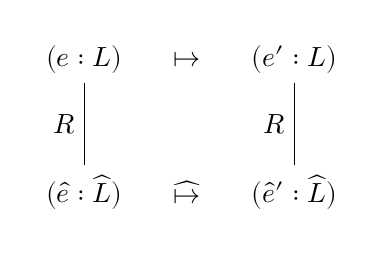
\begin{tikzpicture}[ampersand replacement=\&]

\matrix (m) [matrix of math nodes,row sep=3em,column sep=4em,minimum width=2em]
{ (\Ce : \C) \& (\Ce' : \C) \\
  (\Ae : \A) \& (\Ae' : \A) \\
} ;
\path

(m-1-1) 
edge [white]
node [black] {$\Csteps$} 
(m-1-2)

(m-2-1) 
edge [white]
node [black] {$\Asteps$}
(m-2-2)

(m-1-1) 
edge
node [left] {$R$} 
(m-2-1)

(m-1-2) 
edge
node [left] {$R$} 
(m-2-2)

;

\end{tikzpicture}\end{center}\end{donotbreak}

This picture takes place at some point in the analysis process.
$\Ce$ is the current program (possibly the result of running the base program for a little while).
$\Ae$ is a valid abstraction of $\Ce$, where this validity is expressed by some relation $R$ holding between $\Ce$ and $\Ae$.
$\Ce'$ is some next state of execution of $\Ce$, and likewise for $\Ae$/$\Ae'$.
In order to be a correct analysis, it must be guaranteed that $\Ce'$ and $\Ae'$ will be related.
The logical structure of the picture, which states the correctness of the analysis, is given by:
\begin{equation*}
∀ (\Ce,\Ce' : \C ) (\Ae,\Ae' : \A), (\Ce R \Ae) ∧ (\Ce \Csteps \Ce') ∧ (\Ae \Asteps \Ae') ⇒  (\Ce' R \Ae')
\end{equation*}
The \emph{meaning} of the analysis is entirely subject to the relation $R$ which relates the abstract to the concrete.

% }}}

% Galois Connections {{{
\subsection{Galois Connections}
\label{section:Background:GaloisConnections}

The AI setting can be elegently simplified and enriched through the use of \emph{galois connections}.
Galois connections serve as a unifying framework for establishing the “relationship between $\C $ and $\A$” mentioned in the previous section.

A galois connection between two posets (sets with a partial order) $\C$ and $\A$ is notated $\C\galois{α}{γ}\A$ and contains:
\begin{itemize}
\item $(α : \C → \A)$ where $α$ is monotonic
\item $(γ : \A → \C )$ where $γ$ is monotonic
\item A proof that $(γ ∘ α)$ is expansive: $∀ (x : \C ), x ⊑ γ(α(x))$
\item A proof that $(α ∘ γ)$ is contractive: $∀ (y : \A), α(γ(y)) ⊑ y$
\end{itemize}
The last two properties can be succinctly stated as $(α ∘ γ ⊑ id ⊑ γ ∘ α)$\footnote{
  This uses the logical monotonicity relation $f ⊑ g ⇔  (x ⊑ y ⇒  f(x) ⊑ g(y))$ for the function space.
}.
Equivalent to all four properties is the property $x ⊑ γ(y) ⇔  α(x) ⊑ y$.

The expansive property corresponds to \emph{soundness}, and the contractive property corresponds to \emph{tightness}.
A sound analysis gives results you can trust.  
A tight analysis promises to be the “best” analysis possible.

\paragraph{Example:}
Given a galois connection $\C\galois{α}{γ}\A$, there exists a galois connection $(\C → \C)\galois{α'}{γ'}(\A → \A)$ where:
\begin{align*}
α'(f : \C → \C) &≔ α ∘ f ∘ γ \\
γ'(g : \A → \A) &≔ γ ∘ g ∘ α \\
\end{align*}

\paragraph{Example:} 
The language $(\PM(ℤ),+,*)$ forms a galois connection with the language $(\PM(\{ EVEN, ODD \}),∧,∨)$ where:
\begin{align*}
α(zs : \PM(ℤ))               &≔ ⋃ \{ \{ EVEN  \;|\; ∃ z ∈ zs ∧ Even(z) \},  \{ ODD   \;|\; ∃ z ∈ zs ∧ Odd(z) \} \} \\
γ(ts : \PM(\{ EVEN, ODD \})) &≔ ⋃ \{ \{ z ∈ ℤ \;|\; EVEN ∈ ts ∧ Even(z) \}, \{ z ∈ ℤ \;|\; ODD ∈ ts ∧ Odd(z) \} \} \\
\end{align*}

Galois connections simplify the AI framework by using $x ⊑ γ(y)$ or (equivalently) $α(x) ⊑ y$ as the relation $(x R y)$.
Galois connections are a natural and general way of placing partial orders \emph{on sets themselves}.
$x ⊑ γ(y)$ can be seen as a heterogenous extension of $x ⊑ y$ when $(x : A)$ and $(y : B)$ live in different sets. 
This heterogenous order is given meaning when there exists a galois connection $A\galois{α}{γ}B$.
One can also think of galois connections as something like an isomorphism, but with a weaker round-trip property.
(An isomorphism would require $α ∘ γ = id = γ ∘ α$.)

Using galois connections, the AI framework introduced in the previous section can be re-stated. In the AI framework, an analysis for $\Ce$ is:
\begin{itemize}
\item 
  An abstract language $\A$.
\item 
  A galois connection $\C\galois{α}{γ}\A$.
\item 
  An abstract version of the $\Csteps$ relation: $(\Asteps : \A × \A → Prop)$
\item 
  A way to explore every state reachable by $\Ae$ under $\Asteps$.
  This often requires $\A$ to be finite.
\end{itemize}
The overall approach is summarized in the following picture:
\begin{donotbreak}
\begin{center}
\begin{tabular*}{0.66\textwidth}{@{\extracolsep{\fill}} c c}

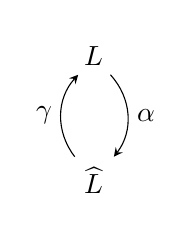
\begin{tikzpicture}[ampersand replacement=\&]
\matrix (m) [matrix of math nodes,row sep=3em,column sep=4em,minimum width=2em]
{ \C \\
  \A \\
} ;
\path [-stealth]

(m-1-1) 
edge [bend left=40]
node [right] {$α$} 
(m-2-1)

(m-2-1) 
edge [bend left=40]
node [left] {$γ$} 
(m-1-1)

;
\end{tikzpicture}

&

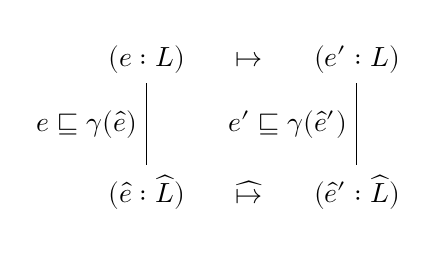
\begin{tikzpicture}[ampersand replacement=\&]
\matrix (m) [matrix of math nodes,row sep=3em,column sep=4em,minimum width=2em]
{ (\Ce : \C) \& (\Ce' : \C) \\
  (\Ae : \A) \& (\Ae' : \A) \\
} ;
\path

(m-1-1) 
edge [white]
node [black] {$\Csteps$} 
(m-1-2)

(m-2-1) 
edge [white]
node [black] {$\Asteps$}
(m-2-2)

(m-1-1) 
edge
node [left] {$\Ce ⊑ γ(\Ae)$} 
(m-2-1)

(m-1-2) 
edge
node [left] {$\Ce' ⊑ γ(\Ae')$} 
(m-2-2)

;
\end{tikzpicture}

\end{tabular*}
\end{center}
\end{donotbreak}

As before, the logical structure of the picture is given by:
\begin{equation*}
∀ (\Ce,\Ce' : \C ) (\Ae,\Ae' : \A), (\Ce ⊑ γ(\Ae)) ∧ (\Ce \Csteps \Ce') ∧ (\Ae \Asteps \Ae') ⇒  (\Ce' ⊑ γ(\Ae'))
\end{equation*}
The statement of this property can be simplified further as $\Csteps ⊑ γ(\Asteps)$.
This uses the definition of galois connections for function spaces shown in a previous example.

Using a galois connection $\C\galois{α}{γ}\A$ and abstract step function $\Asteps ⊑ γ(\Csteps)$, the analysis story becomes simplified even further:
\begin{itemize}
\item Translate $(\Ce : \C)$ to $(α(\Ce) : \A)$
\item Explore all abstract states $\Ae'$ states reachable from $α(\Ce)$.
\item All reachable concrete states are summarized by projecting each $γ(\Ae')$ back to $\C$.
\end{itemize}

The galois connection framework simultaneously guarantees the \emph{soundness} and \emph{tightness} of this method.
Soundness tells us that if we abstract, take an abstract step, and then concretize, then the result is an approximation of taking a concrete step.
Soundness tells us that we can trust the results of the analysis.
\begin{donotbreak}
\begin{center}

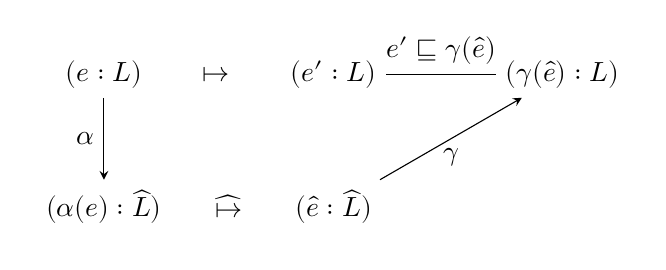
\begin{tikzpicture}[ampersand replacement=\&]
\matrix (m) [matrix of math nodes,row sep=3em,column sep=4em,minimum width=2em]
{ (\Ce : \C)    \& (\Ce' : \C) \& (γ(\Ae) : \C) \\
  (α(\Ce) : \A) \& (\Ae : \A)  \&               \\
} ;
\path [-stealth]

(m-1-1) 
edge
node [left] {$α$} 
(m-2-1)

(m-2-1) 
edge [white]
node [black] {$\Asteps$}
(m-2-2)

(m-2-2)
edge
node [below] {$γ$} 
(m-1-3) 

(m-1-1) 
edge [white]
node [black] {$\Csteps$} 
(m-1-2)

;

\path

(m-1-2)
edge
node [above] {$\Ce' ⊑ γ(\Ae)$}
(m-1-3)

;
\end{tikzpicture}

\end{center}
\end{donotbreak}


Tightness tells us that if we concretize, take a concrete step, and then abstract, then the result must be just as precise as taking an abstract step.
Tightness tells us that our abstract step function isn't losing precision unnecessarily, and that our abstract step $\Asteps$ is provably as strong as possible.
\begin{donotbreak}
\begin{center}

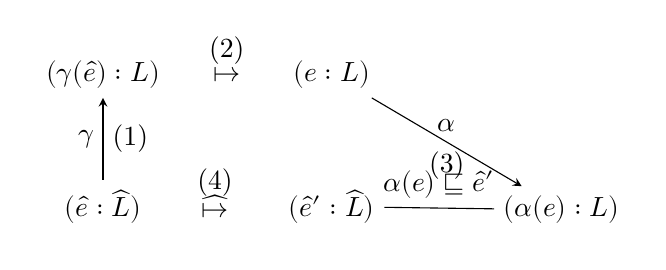
\begin{tikzpicture}[ampersand replacement=\&]
\matrix (m) [matrix of math nodes,row sep=3em,column sep=4em,minimum width=2em]
{ (γ(\Ae) : \C) \& (\Ce : \C) \&                \\
  (\Ae : \A)    \& (\Ae' : \A) \& (α(\Ce) : \C) \\
} ;
\path [-stealth]

(m-2-1) 
edge
node [left] {$γ$} 
node [right] {(1)} 
(m-1-1)

(m-1-1) 
edge [white]
node [black,above] {(2)}
node [black] {$\Csteps$}
(m-1-2)

(m-1-2)
edge
node [above] {$α$} 
node [below] {(3)}
(m-2-3) 

(m-2-1) 
edge [white]
node [black] {$\Asteps$} 
node [black,above] {(4)}
(m-2-2)

;

\path

(m-2-2)
edge
node [above] {$α(\Ce) ⊑ \Ae'$}
(m-2-3)

;
\end{tikzpicture}

\end{center}
\end{donotbreak}




% }}}

% Control Flow Analysis {{{
\subsection{Control Flow Analysis}
\label{section:Background:ControlFlowAnalysis}

Control flow analysis is a class of analysis which is particularly important for higher-order languages.
In non-higher-order languages, it is useful to distinguish control-flow from data-flow.
The control flow of the program is a graph of what functions are called from where.
The data flow of a program is a mapping of which values can flow to which variables.
Traditionally one performs a control-flow analysis first, to find out which functions are called, and a data-flow analysis second, using the results of the control flow analysis.

In higher-order languages, data-flow and control-flow are tightly coupled.
Before you can tell which functions will be called, you need to know how values flow, because functions are themselves values.

We note that the distinction between “higher-order” languages and “non-higher-order” languages is a red herring.
Functions can be passed as values in C using function pointers, and object-oriented languages enjoy a similar circularity between control- and data- flow due to method dispatch.
You can read these statements as saying “all languages are higher order, and thus all languages need higher order control flow analysis”.
Or you can read them as saying “all languages are higher order, and we've done just fine without higher oder control flow analysis so far”.
The real distinction is in the code that you end up analysing.

We build on the tradition of control flow analysis (CFA) pioneered by Shivers, as well as recent refinements of CFA developed by Might and Van Horn.
In this tradition, the result of a control flow analysis is closer to what one would think of as a data-flow analysis, only the process accounts for higher order flow.
0CFA, the most basic control flow analysis, merely computes the set of values which might flow to a particular variable.
kCFA is a suite of context sensitive extensions to 0CFA for which functions are analyzed separately for each possible calling context.
We use 0CFA as the example analysis in this paper.
However our framework, and our implementation of it, scale to the full range of context sensitive control flow analyses.

% }}}

% Monads {{{
\subsection{Monads}
\label{section:Background:Monads}

A basic familiarity with the concept of monads will be necessary for understanding this paper.
Some find it useful to review the concept of functor before learning about monads. 
We adopt this approach for our brief explanation of monads.

A type $(F : Set → Set)$ is called a \emph{functor} if one can:
\begin{itemize}
\item Define $map : ∀ (A, B : Set), (A → B) → (F(A) → F(B))$
\item Prove $map(id) = id$, where $id$ is the identity function $(λ(x) → x)$
\item Prove $map (g ∘ f) = map(g) ∘ map(f)$
\end{itemize}

\paragraph{Example:} 
Lists are functors, where $map$ is defined:
\begin{align*}
    map(f)(xs) ≔ &\case(xs):           \\
          Nil    &→ Nil                \\
         x ∷ xs' &→ f(x) ∷ map(f)(xs') \\
\end{align*}

\paragraph{Example:} $map(isEven)([1, 2, 3, 4]) = [False, True, False, True]$

Likewise a type $(ℳ  : Set → Set)$ is called a \emph{monad} if one can:
\begin{itemize}
\item Define $extend : ∀ (A, B : Set), (A → ℳ (B)) → (ℳ (A) → ℳ (B))$
\item Prove unit and associativity laws (not mentioned here).
\end{itemize}
The only difference from the definition of functor is in the the first argument.
For monads, this argument is allowed to be a \emph{monadic} $(A → ℳ (B))$, rather than a pure function $(A → B)$.

\paragraph{Example:} Lists are monads, where $extend$ is defined:
\begin{align*}
    extend(f)(xs) ≔ &\case(xs):              \\
                Nil &→ Nil                   \\
            x ∷ xs' &→ f(x) ⧺ extend(f)(xs') \\
\end{align*}

\paragraph{Example:} 
$extend(λ(x) → [x + 1, x - 1])([10, 100]) = [9, 11, 99, 101]$

$extend$ for lists can also be understood as $concat$ followed by $map$:
\paragraph{Example:} 
\begin{align*}
extend(f)([10, 100]) &= concat(map(f)([10, 100]))    \\
                     &= concat([[9, 11], [99, 101]]) \\
                     &= [9, 11, 99, 101]             \\
\end{align*}
For all monads, it is equivalent to define $return$, $map$ and $join$, where:
\begin{equation*}
join : ∀ (A : Set), ℳ (ℳ (A)) → ℳ (A)
\end{equation*}
As we have just seen, $join$ for the list monad is just $concat$.

% }}}

% Monad Transformers {{{
\subsection{Monad Transformers}
\label{section:Background:MonadTransformers}

Monad transformers are functions between monads.
Where a monad $ℳ $ will have type $Set → Set$, a monad transformer $𝒯$ will have type $(Set → Set) → (Set → Set)$.

Monad transformers are used to extend an existing monad to support another effect.
The three monads used in this work are the state monad, powerset monad, and the identity monad.
The state monad is notated $\SM(𝓈)$ (carrying a single cell of type $𝓈$), the powerset monad is notated $\PM$, and the identity is notated $ID$.
The state and powerset monad transformer equivalents are notated $\ST(𝓈)(ℳ )$ and $\PT(ℳ )$ where $ℳ $ is the underlying monad.
The state monad has $get$ and $put$ effects, whereas the powerset monad has a $nondeterminism$ effect.
The transformer versions of both of these monads allow you to combine effects piecewise.

\paragraph{Example:}
$\ST(ℤ)(\PT(ID))$ is a monad which has $get$ and $put$ effects for a single cell of integer state, in addition to nondeterminism effects.

The definitions, details and proofs of all monads used in our work are given in section \ref{section:Proofs}.

% }}}

% }}}

% Monadic AAM {{{

\section{Monadic AAM}
\label{section:MonadicAAM}
%* Monadic AAM
%  - 0CFA Before Monads
%  - 0CFA After Monads
%  - Recovering the Previous Analysis


Monadic abstract interpretation[Sergey et al. PLDI 2013] demonstrated that abstract interpreters can be built using a monadic abstraction.
We build directly on the intuition of this work: monadic interpreters are easier to develop than state machines.
However, our approach takes this idea further in pursuit of a more compositional framework.

First we demonstrate a simple 0CFA analysis on CPS-IF using classic AAM.
The CPS-IF language is introduced in section \ref{CPS}.
We repeat the definition here for convenience.
\begin{align*}
x,y,k : Var  &⩴ ..variables..                                            \\
b,i,l : Lit  &⩴ ℤ ∪ 𝔹                                                    \\
  f,g : Lam  &⩴ \lam(x) → e \;|\; \lam(x,k) → e                          \\
    a : Atom &⩴ x \;|\; l \;|\; f \;|\; op(a)                            \\
   op : Op   &⩴ \add \;|\; \sub \;|\; \gez                               \\
    e : Call &⩴ \iif(a)\{e\}\{e\} \;|\; a(a) \;|\; a(a,a) \;|\; \halt(a) \\
\end{align*}



The abstract semantics of 0CFA will track literals (including lambdas) that appear in the program text.
For integers that do not appear in the program text, the analysis uses a single token $INT$ which conservatively approximates any possible integer.
We note that many more abstractions of integers are possible, like range analysis or relational integer analysis.
These decisions do not interfere with AAM or abstract control, so we do not discuss them for simplicity.

Formally, the state space $Σ$ for the abstract machine of the abstract semantics is defined as:
\begin{align*}
v : \AVal   &⩴ l \;|\; f \;|\; INT \\
σ : \AStore &≔ Var → \PM(\AVal)    \\
Σ           &≔ \PM(Call × \AStore) \\
\end{align*}

Because there are finite many literals in the program text, we can claim that $\AVal$ and $\AStore$ are finite.

The abstract semantics for $Σ$ comes in two parts.  
First we define a \emph{denotation function} $𝒜 $ for $Atom$ expressions.
\begin{align*}
𝒜                            &: \AStore × Atom → \PM(\AVal) \\
𝒜 (σ,x)                      &≔ σ(x)                        \\
𝒜 (σ,l)                      &≔ \{ l \}                     \\
𝒜 (σ,\add a) | 𝒜 (σ,a) ⊑ INT &≔ \{ \INT \}                  \\
𝒜 (σ,\sub a) | 𝒜 (σ,a) ⊑ INT &≔ \{ \INT \}                  \\
𝒜 (σ,\gez a) | 𝒜 (σ,a) ⊑ INT &≔ \{ \TRUE , \FALSE \}        \\
𝒜 (σ,\lam(x) → e)            &≔ \{ \lam(x) → e \}           \\
𝒜 (σ,\lam(x)(k) → e)         &≔ \{ \lam(x)(k) → e \}        \\
\end{align*}



Second we define a \emph{step relation} (as a function) $𝒞$ for $Call$ expressions.
\begin{align*}
𝒞                        : &Call × \AStore → \PM(Call × \AStore)                                            \\
𝒞(\iif(a)\{e₁\}\{e₂\},σ) ≔ &\{ (e,σ)                                                                        \\
                           &|\; e ∈ ⋃ \{ \{ e₁ \;|\; \TRUE ∈ 𝒜 (σ,a) \}, \{ e₂ \;|\; \FALSE ∈ 𝒜 (σ,a) \} \} \\
                           &\}                                                                              \\
          𝒞(a₁(a₂,a₃),σ) ≔ &\{ (e,σ')                                                                       \\
                           &|\; (\lam(x)(k) → e) ∈ 𝒜 (σ,a₁)                                                 \\
                           &|\;             v₂ ∈ 𝒜 (σ,a₂)                                                   \\
                           &|\;             v₃ ∈ 𝒜 (σ,a₃)                                                   \\
                           &|\;             σ' ≔ σ ⊔ [x ↦ v₂] ⊔ [k ↦ v₃]                                    \\
                           &\}                                                                              \\
           𝒞(\halt(a),σ) ≔ &\{ (\halt(a),σ) \}                                                              \\
\end{align*}

(We omit the $(a₁(a₂))$ case. It is directly analogous to $(a₁(a₂,a₃))$).

The complete analysis of an expression $e$ is defined as the least fixed point of a \emph{collection semantics} for the relation $𝒞$:
\begin{align*}
\text{analysis} ≔ μ(Σ) → \{(e,⊥)\} ⊔ 𝒞^{⋆}(Σ)
\end{align*}
where
\begin{align*}
𝒞^{⋆}    &: \PM(Call × \AStore) → \PM(Call × \AStore) \\
𝒞^{⋆}(Σ) &≔ ⋃ \{ 𝒞(e,σ) | (e,σ) ∈ Σ \}                  \\
\end{align*}
The collecting semantics tracks all states that the program could be in rather than just the final states.

The first insight in monadic abstract interpretation is to abbreviate the definitions of $𝒜 $ and $𝒞$ monadic state rather than explicit state-passing-style.
At this point, the monad “trick” is nothing more than a technique to simplify the definition of $𝒜 $ and $𝒞$.

We use a powerset monad underneath a state monad transformer to write the analysis in monadic style.
\begin{align*}
ℳ     &: Set → Set                  \\
ℳ (a) &≔ \ST(\AStore)(\PM)(a)       \\
ℳ (a) &≔ \AStore → \PM(a × \AStore) \\
\end{align*}

The full definitions of the monads (and their proofs) used throughout this paper are defered to section \ref{Proofs}.
Because monad transformers are just fancy names for simple types, we write the equivalent simple type underneath definitions which use monad transformer.

The monadic conversion of $𝒜 $ interacts with the store $σ$ using get and put operations.
\begin{align*}
𝒜_{m}                 &: Atom → ℳ (\PM(\AVal))                         \\
𝒜_{m}(x)              &≔ \ddo                                          \\
                      &σ ← \getstore                                   \\
                      &\return(σ(x))                                   \\
𝒜_{m}(l)              &≔ \return(\{l\})                                \\
𝒜_{m}(add1(a))        &≔ \ddo                                          \\
                      &v ← 𝒜_{m}(a)                                    \\
                      &\return(\{\INT \;|\; ∃ i ⊑ \INT ∈ v\})          \\
𝒜_{m}(sub1(a))        &≔ \ddo                                          \\
                      &v ← 𝒜_{m}(a)                                    \\
                      &\return(\{\INT \;|\; ∃ i ⊑ \INT ∈ v\})          \\
𝒜_{m}(gez(a))         &≔ \ddo                                          \\
                      &v ← 𝒜_{m}(a)                                    \\
                      &\return(\{\TRUE, \FALSE \;|\; ∃ i ⊑ \INT ∈ v\}) \\
𝒜_{m}(\lam(x)(k) → e) &≔ \return(\{\lam(x)(k) → e\})                   \\
\end{align*}


The monadic conversion of $𝒞$ doesn't use monadic actions directly.
\begin{align*}
                     𝒞_{m} &: Call → ℳ (Call)                                                  \\
𝒞_{m}(\iif(a)\{e₁\}\{e₂\}) &≔ \ddo                                                             \\
                           &vP ← 𝒜_{m}(a)                                                      \\
                           &v ← \liftpowerset(vP)                                              \\
                           &b ← \coercebool(v)                                                 \\
                           &\return(\{ \text{if}\; b\; \text{then}\; e₁\; \text{else}\; e₂ \}) \\
          𝒞_{m}(a₁(a₂,a₃)) &≔ \ddo                                                             \\
                           &vP ← 𝒜_{m}(a₁)                                                     \\
                           &v ← \liftpowerset(vP)                                              \\
                           &(\lam(x)(k) → e) ← \coercefun(v)                                   \\
                           &vP₂ ← 𝒜_{m}(a₂)                                                    \\
                           &vP₃ ← 𝒜_{m}(a₃)                                                    \\
                           &σ ← \getstore                                                      \\
                           &\putstore(σ ⊔ [x ↦ vP₂] ⊔ [k ↦ vP₃])                               \\
                           &\return(e)                                                         \\
\end{align*}

The “effects” in $𝒞_{m}$ happen in its calls to $𝒜_{m}$, $\liftpowerset$, $\coercebool$ and $\coercefun$.
$𝒜_{m}$ will have state effects and $\liftpowerset$, $\coercebool$ and $\coercefun$ will have nondeterminism effects.

$\liftpowerset$, $\coercebool$ and $\coercefun$ use the nondeterminism monadic effect and are defined as follows:
\begin{align*}
                 \liftpowerset &: 𝒫 (a) → ℳ (a)                        \\
\liftpowerset(\{x₁, ..., x₂\}) &≔ ⋃ \{return (x₁), ... , return (x₂)\} \\
                                                                       \\
                   \coercebool &: \AVal → ℳ  (𝔹 )                      \\
               \coercebool (b) &≔ return(b)                            \\
              \coercebool (\_) &≔ ⊥                                    \\
                                                                       \\
                    \coercefun &: \AVal → ℳ  (Lam)                     \\
                \coercefun (f) &≔ return(f)                            \\
               \coercefun (\_) &≔ ⊥                                    \\
\end{align*}


The monadic abstraction leads to a simplified definition of the analysis.
This simplification becomes much more apparent as a state space grows to have more than two states.
Metafunctions which interact with only one state component can be written generically to support any state space which has that component.

As before, we must complete the analysis by building an abstract machine transition function:
\begin{align*}
𝒞_{m}^{⋆}    &: \PM(Call × \AStore) → \PM(Call × \AStore) \\
𝒞_{m}^{⋆}(Σ) &≔ ⋃ \{ 𝒞_{m}(e)(σ) \;|\; (e,σ) ∈ Σ \}          \\
\end{align*}

Our current definition of $ℳ $ recovers exactly the analysis we wrote before.
On top of the convenience of writing things monadically, our insight and contribution is twofold:
\begin{itemize}
\item State spaces $Σ$ can be defined and proven correct compositionally using monad transformers.
\item $𝒞_{m}$ can be written generic to a monadic effect signature, rather than a specific monad.
      Multiple different monads can be shown to meet this signature, and swapping the monad allows one to tune the flow and path sensitivity of an analysis.
\end{itemize}

% }}}

% Abstract Control {{{
\section{Abstract Control}
\label{section:AbstractControl}
%* Abstract Control
%  - Axiomatize monadic interface
%  - Build interface from legos
%  - Swapping the legos gives you PS - FS - FI

The current instantiation of ℳ  in our example happens to give a flow-sensitive path-sensitive analysis.
Consider a reordering of powerset and state monad transformers:
\begin{align*}
ℳ     &: Set → Set                  \\
ℳ (a) &≔ \PT(\SM(\AStore))(a)       \\
ℳ (a) &≔ \AStore → \PM(a) × \AStore \\
\end{align*}
As before, we must convert between monadic actions and abstract state space transitions to achieve an analysis:
\begin{align*}
𝒞_{m}^{⋆}       &: \PM(Call) × \AStore → \PM(Call) × \AStore                                              \\
𝒞_{m}^{⋆}(cP,σ) &≔ (\{ e' \;|\; e' ∈ π₁(𝒞_{m}(e))(σ) \;|\; e ∈ e\PM \}, ⋃ \{ π₂(𝒞(e))(σ) \;|\; e ∈ cP \}) \\
\end{align*}
This instantiation of $ℳ $ and $𝒞_{m}^{⋆}$ yields a flow-insensitive path-insensitive analysis.
For the same monad $ℳ $, we can change the definition of $𝒞_{m}^{⋆}$ to achieve a flow-sensitive path-insensitive analysis:
\begin{align*}
𝒞_{m}^{⋆}    &: \PM(Call × \AStore) → \PM(Call × \AStore)                             \\
𝒞_{m}^{⋆}(Σ) &≔ \{ (e',π₂(𝒞_{m}(e))(σ)) \;|\; e' ∈ π₁(𝒞_{m}(e))(σ) \;|\; (e,σ) ∈ Σ \} \\
\end{align*}
By altering the monad behind the abstraction, we are able to tune the path sensitivity of the analysis.
For the path-insensitive monad, we were able to further alter the resulting state space $Σ$ to tune the flow sensitivity of the analysis.

% Talk about monad transformers as building blocks.  How these computations (and their proofs) fall out fully compositional components.

% }}}

% Intensional Optimizations {{{
\section{Intensional Optimizations}
\label{section:IntensionalOptimizations}
% * Intensional Optimizations
%   - Garbage Collection
%   - MCFA

Up to this point we have factored the abstract control properties of static analysis behind a common interface.  
Now we show how to implement two intentional optimizations, abstract garbage collection and mcfa, in a completely general setting.

\paragraph{Abstract Garbage Collection}
Abstract garbage collection is an optimization technique in abstract interpretation where unreachable abstract addresses are pruned from the state space.
This is analagous to “real” garbage collection, where unreachable pointers are reclaimed for space efficiency.
However, in abstract semantics, live addresses are \emph{re-used} as part of the sound and finite approximation of an infinite address space.
When a live address present in the heap must be used for allocation, a static analysis is forced to lose precision.
Abstract garbage collection exploits the realization that these live addresses can be collected before they are reallocated, resulting in no loss of precision.

For a generic implementation of garbage collection we assume an arbitrary $ℳ $ that has $get$, $put$ and nondeterminism effects.
This allows us to change the flow and path sensitivity of the garbage collection without having to reimplement that analysis.
\begin{align*}
   gc &: Call → ℳ (1)                                   \\
gc(e) &≔ \ddo                                           \\
      &σ ← \getstore                                    \\
      &𝓉₀ ← \touchedcall(e)                             \\
      &\llet 𝓉 ≔ μ(𝓉) → 𝓉 ⊔ \touchedvar(𝓉)              \\
      &σ ← \getstore                                    \\
      &\putstore(⋃ \{ [x ↦ vP] | x ∈ 𝓉 ∧ σ(x) = vP \} ) \\
\end{align*}

This is literally the implementation of \emph{concrete} garbage collection, but with control properties abstracted behind a monad.
When instantiated with path-sensitive, flow-sensitive or flow insensitive monads, we can recover the appropriate version of control for abstract garbage collection.

In the original AAM paper, abstract garbage collection is described using a path-sensitive CESK* machine.
Later in the paper, the path-sensitive CESK* machine is abstracted to use a single global store, which yields a less precise but more tractable analysis.
However, the single-store variant of the analysis requires one to repeat the “instrument then abstract” design process for abstract garbage collection.
By abstracting control and exposing it as an orthogonal tuning knob, we are able to design flow and path sensitive variants of garbage collection at once.

\paragraph{MCFA}

MCFA is an optimization that improves the asymptotic complexity of context-sensitive control flow analyses for functional languages.
Context sensitive analysis were shown to be exponential for functional analyses, yet polynomial for OO analysis, creating an apparent paradox.
MCFA resolves this paradox by identifying the difference in context sensitive analyses and porting the polynomial behavior from OO to functional analyses.
The key insight of MCFA is to use packed, copied closures rather than linked closures in the abstract semantics.
Like garbage collection, using packed rather than linked closures is a simple optimization a compiler or concrete interpreter might use to increase performance.
Like \emph{abstract} garbage collection, transporting this simple idea from concrete to abstract interpreters reveals a surprising analysis optimization.

The examples so far have covered 0CFA, a context insensitive analysis.
Before discussing MCFA, we add context sensitivity to our example analysis.

To incorporate context sensitivity into the analysis we do the following:
\begin{itemize}
\item Add another state space component to $Σ$ for environments: $\AEnv$.
      This environment will track which calling function is responsible for binding a given parameter.
\item Capture this environment when evaluating $λ$ expressions, just like a concrete interpreter would for concrete environments.
\item Add another state space component which tracks the program points visited so far by the program: $\ATime$.
\item When interpreting a command $𝒞_{m}(e)$, move time forward by adding $e$ to the list of program points visited.
\item When calling a function, record the current time next to the function arguments in the environment.
\end{itemize}
These steps have the effect of re-analyzing a function twice if it is called from two separate places.

Changing the state space two have two new components is achieved by adding two more state effects two our monad, one for $\AEnv$ and one for $\ATime$:
\begin{align*}
  ρ : \AEnv &≔ Var ⇀ \ATime                              \\
σ : \AStore &≔ (Var,\ATime) → \PM(\AVal)                 \\
 τ : \ATime &≔ Call \;\text{(the last program location)} \\
 f,g : Lam  &⩴ \lam(x) → e \;|\; \lam(x,k) → e           \\
  clo : Clo &⩴ ⟨f, ρ⟩                                    \\
  v : \AVal &⩴ l \;|\; clo \;|\; INT                     \\
\end{align*}

Capturing the environment when evaluating $λ$ expressions is a simple monadic action:
\begin{align*}
𝒜_{m}                &: Atom → ℳ (\PM(\AVal))      \\
                 ... &                             \\
𝒜_{m}(\lam(x) → e)   &≔ \ddo                       \\
                     &ρ ← \getenv                  \\
                     &\return (⟨\lam(x) → e, ρ⟩)   \\
𝒜_{m}(\lam(x,k) → e) &≔ \ddo                       \\
                     &ρ ← \getenv                  \\
                     &\return (⟨\lam(x,k) → e, ρ⟩) \\
                 ... &                             \\
\end{align*}
This is the “linked” implementation of closures, which MCFA will replace with a packed version.

Moving abstract time forward is a simple update of the $\ATime$ state to be the current call expression:
\begin{align*}
   𝒞_{m}' &: Call → ℳ (Call) \\
𝒞_{m}'(e) &≔ \ddo            \\
          &\puttime(e)       \\
          &𝒞_{m}(e)          \\
\end{align*}

Calling a function now uses time as an address for storing values in $\AStore$.
\begin{align*}
           𝒞_{m} &: Call → ℳ (Call)                            \\
             ... &                                             \\
𝒞_{m}(a₁(a₂,a₃)) &≔ \ddo                                       \\
                 &vP ← 𝒜_{m}(a₁)                               \\
                 &v ← \liftpowerset(vP)                        \\
                 &(⟨\lam(x)(k) → e, ρ⟩) ← \coercefun(v)        \\
                 &vP₂ ← 𝒜_{m}(a₂)                              \\
                 &vP₃ ← 𝒜_{m}(a₃)                              \\
                 &σ ← \getstore                                \\
                 &τ ← \gettime                                 \\
                 &\putenv(ρ[x ↦ τ][k ↦ τ])                     \\
                 &\putstore(σ ⊔ [(x,τ) ↦ vP₂] ⊔ [(k,τ) ↦ vP₃]) \\
                 &\return(e)                                   \\
             ... &                                             \\
\end{align*}

Now that we have a context sensitive analysis, MCFA is implemented by creating a new packed environment, rather than just linking with the current environment:
\begin{align*}
𝒜_{m}                &: Atom → ℳ (\PM(\AVal)) \\
                 ... &                        \\
𝒜_{m}(f)             &≔ \ddo                  \\
                     &\llet ys ≔ \operatorname{free-vars}(f)        \\
                     &vs ← map^{⋆}(lookup)(ys)                      \\
                     &ρ ← \{ y ↦^{⋆} v \;|\; (y,v) ∈ zip(ys, vs) \} \\
                     &\return(⟨f,ρ⟩)                                \\
                 ... &                        \\
\end{align*}


Like abstract garbage collection, our implementation of MCFA is tunable from one implementation which has abstracted control through a monad.
Flow and path sensitive variants of MCFA fall out of a simple rearranging of the monad transformer stack.

% }}}

% Correctness {{{

\section{Correctness}
\label{section:Correctness}
% * Correctness
%   - All Legos give correct analyses
%   - Nondeterminism MT
%   - Monad Transformers relate to state machine functors.
%   - Galois connections with functors for α γ maps


The key advantage to our framework is that the proofs of correctness for constructed analyses are constructed compositionally and derived automatically.
The proofs are compositional because they are established at the level of monad transformers, not hard-coded for a full monad stack.
The proofs are derived automatically through the galois-functorality of the monad transformers we use; they transport galois connections in addition to monadic actions.
Given these proofs, along with an argument about monotonicity of the monadic semantics, we can establish a proof of galois connection for any given interpreter instantiation.

To relate back to abstract machine semantics, we establish a galois connection between monadic actions in $ℳ $ and transitions functions for \emph{some} abstract state space $𝒮𝒮$.
This abstract state space is constructed from the monad transformer stack, although some transformer stacks support multiple abstract state spaces.
This property is notated $(A → ℳ (B))\galois{α}{\gamma}(𝒮𝒮(A) → 𝒮𝒮(B))$.
We call a particular monad $ℳ $ which enjoys this property a \emph{small-step monad}.
Likewise, we call a monad transformer $𝒯$ which enjoys \emph{transports} this property a \emph{small-step monad transformer}.

In our framework we prove that not only are $\ST$ and $\PT$ monad transformers, they're small-step monad transformers.
This means that for any stack of interleaving $\ST$ and $\PT$ monad transformers, one can construct the necessary galois connection back to small step semantics.

We prove that $\ST(𝓈)(\PM) ⊑ \PT(\SM(𝓈))$.
These monad interleavings correspond to path-sensitivity and path-insensitivity respectively.

For the $\PT(\SM(𝓈))$ monad, we show two galois connections are possible: one to the state space $\PM(\_ × 𝓈)$ and one to the state space $(\PM(\_) × 𝓈)$.
These choices for galois connection correspond to flow-sensitivity and flow-insensitivity respectively.

Independent of language or application we have proven:
\begin{align*}
flow-insensitive ⊑ flow-sensitive path-insensitive ⊑ flow-sensitive 
\end{align*}

A given concrete semantics will always use the flow-sensitive path-sensitive monad.
Using this bridge we can construct a galois connection between concrete and a flow-insensitive abstract semantics with no added effort.

This table summarizes these results, showing both the monad $ℳ $ and state space $Σ$ which correspond to each analysis:
\begin{center}\begin{tabular}{| c | c | c |}
  \hline Sensitivity      & Path Sensitive                    & Path Insensitive                  \\
  \hline Flow Sensitive   & $ℳ  ≔ S ∘ 𝒫$ \newline $Σ ≔ P ∘ ×$ & $ℳ  ≔ 𝒫 ∘ S$ \newline $Σ ≔ 𝒫 ∘ ×$ \\
  \hline Flow Insensitive & $DNE$                             & $ℳ  ≔ × ∘ 𝒫$ \newline $Σ ≔ × ∘ 𝒫$ \\
  \hline                                                                                          \\
\end{tabular}\end{center}
(We write $S and 𝒫$ to abbreviate the state and nondeterminism monad
transformers, and $× and 𝒫$ to abbreviate the cartesian product and
nondeterminism state space functors.)

In summary, when using our framework, the analysis designer need only prove prove:
\begin{itemize}
\item The semantic step function $𝒞_{m}$ is monotonic.
\item The semantics as written, including intensional optimizations, are correct.
\end{itemize}
After supplying these proofs, the analysis designer enjoys:
\begin{itemize}
\item An automatically derived analysis for their language with abstract control left as a tuning knob.
\item A proof-by-construction of galois connection (soundness and tightness) for the derived analysis.
\item Easy integration of new analysis features, a la. AAM.
\item Single-definition implementation of intensional optimizations like abstract garbage collection or MCFA.
\end{itemize}

% }}}

% Related Work {{{
\section{Related Work}
\label{RelatedWork}
% * Abstract Control:
%   - Johnson and Van Horn. 2014. Abstracting Abstract Control.
%     + Discusses push-down as the missing knob.
%     + Different knob settings for the same knob; hopefully they can be combined.
% * Compositional Analysis Design: Calculational AI:
%   - Cousot. 1999. The calculational design of a generic abstract interpreter.
%     + Works for anything in principle, but hasn't been demonstrated.
%   - Midgaard and Jensen. 2008. A Calculational Approach to Control-flow Analysis by Abstract Interpretation.
%     + Calculation is hard; maybe proof assistants can help with this.
% * New knobs: object sensitivity:
%   - Kastrinis and Smaragdakis. 2013. Hybrid Context-Sensitivity for Points-To Analysis.
% * Using Path Sensitivity: 
%   - Das et al. 2002. ESP: Path-Sensitive Program Verification in Polynomial Time.
\paragraph{Abstract Control}
Johnson and Van Horn recently explored the concept of abstract control in their paper Abstracting Abstract Control (AAC)\cite{AAC}.
In this work, the authors discuss how to recover a pushdown abstraction systematically in the setting of AAM.
Our work is orthogonal, and potentially compatible with theirs: our framework explains compositional analyses, while theirs explains pushdown control abstraction.
We hope for an eventual combination of the two techniques, and see this as a ripe area for combination of results.

As far as the question “what is abstract control?”, it appears that we paint a similar picture as Johnson and Van Horn in AAC.
In both works, abstract control has something to do with the fixpoint iteration of the semantic step function, and is noted as lacking in classic AAM.
Our work gives one possible definition for what abstract control is: it's the control effects used by an interpreter, coupled with the way these effects are related to abstract machines.

\paragraph{Compositional Approaches}
Another compositional approach to abstract interpretation is described by Cousot and Cousot: \emph{calculational abstract interpretation}\cite{CalculationalAI}.
Calculational AI shares a similar philosophy to our work: abstract interpreters should be build piecewise from compositional components.
In calculational AI, analyses are derived from applying a sequence of galois connections.
This contrasts to the approach of designing an analysis first, and manually justifying the galois connection after.
After applying a sequence of galois connections, the analysis designer must \emph{calculate} the computable analysis from the one derived by galois connection composition.

The downfall of calculational AI is in the effort required during the calculation step.
For example, Midgaard and Jensen\cite{Calculational0CFA} describe a calculational derivation of 0CFA, the same analysis described in this work, and it is a difficult process.

While work in calculational AI has seen less success than AAM, we note that the two approaches are actually compatible, and thus tackle different parts of the analysis design process.
AAM is a methodology for splitting the design process to first instrument a concrete semantics, and then systematically abstract.
Both of these steps must be justified with galois connections, and one could use calculation for either.
Our work provides computations and proofs for the second step, the systematic abstraction, but one might happily justify the instrumentation step via calculation.

\paragraph{Tuning Knobs}
Tuning knobs for static analysis are great when they're general enough for a wide range of applications.
For example, the work Kastrinis and Smaragdakis\cite{HybridContextObject} shows how to leave both context-sensitivity and object-sensitivity as orthogonal tuning knobs in an OO analysis.
These knobs have shown to be sufficient for interesting applications like malware detection for Android applications\cite{Apposcopy}.
(\cite{Apposcopy} directly uses the analysis framework described in\cite{HybridContextObject}.)

\paragraph{Path Sensitivity}
Path sensitivity in particular was shown to be profitible and tractable by Das et al.\cite{ESP}.
In this work the authors verify the absence of open/close file handle bugs in the GNU C compiler.
Path sensitivity was crucial achieve the precision needed for their analysis, and their paper describes to to achieve this precision without too much added cost in complexity.
These subtle variants of path sensitivity are important for applying path sensitive analysis in practice.
We do not account for these particular variants of path sensitivity in our framework, although we hope to explore how they fit into our framework in future work.
% }}}

% Future Work {{{
\section{Future Work}
\label{FutureWork}
% * Future Work:
%   - Verified compilation:
%     + CompCert, but whole program analysis, functional languages.
%     + Requires embedding whole framework in proof assistant.
%     + Mechanizing galois connections is hard, because of calculation.
%   - More knobs for analysis:
%     + Lexical Time
%     + Object sensitivity for functional languages.
%   - Denotational variants of MAAM
%     + Picking small-step semantics has consequences.
%     + Add MonadFix to effects, show a memoizing fixpoint is an abstraction of Y.

\paragraph{Fully Verified Compilation}
One direction of future work is to apply our approach to fully verified compilation.
In fully verified compilation, the implementation of a comipler is typically embedded in proof assistant and proven correct all the way down to axioms in a logical system.
This task is difficult due to both the extra rigor required in modelling and the proof engineering required in interacting with proof assistants.
We hope the compositionality of the \emph{correctness} of our approach will apply especially in this setting, because proofs need to be developed and maintained side-by-side with code.

CompCert\cite{CompCert} is perhaps the most well known fully verified compiler to date.
CompCert compiles C programs down to machine code and performs simple local optimizations.
A verified compiler for languages with rich features like objects and first-class functions benefit especially from approaches like AAM and our extension of it.
Whole program analysis has also not been studied yet in the context of fully verified compilation, perhaps because establishing the proof of correctness is too burdensome.
We hope our technique can be extended to support fully verified compilation of whole program analysis for functional programs in the future.

\paragraph{New Tuning Knobs for Analysis}
Another direction for future work is to discover more tuning knobs for analyses which have been missed by frameworks like AAM.
For example, it would be nice if we could account for the pushdown abstraction from Johnson and Van Horn's work on \emph{Abstracting Abstract Control} into our monadic formulation.
Less related to abstract control, we believe there is work to be done in porting object sensitivity to functional language analysis.
We have preliminary results suggesting that object sensitivity becomes lexically scoped time in the functional setting.
Exploring this would uncover yet another useful knob to analysis designers to quickly interate through the analysis design process.

\paragraph{New Semantic Settings}
Our framework small-step abstract machines semantic framework of AAM.
The small-step setting is convenient, but it has less-well understood consequences when it serves as the basis for abstract interpretation.

For example, we can imagine a more denotational variant of this work where we relate our interpreters to a denotational space rather than state machines.
We have preliminary results suggesting that this can be done by allowing our monadic interpreter to be recursive.
When this is done, the meaning of the program is not given by an external fixpoint of the step function, but rather directly through the denotation of recursion.
To recover an analysis, one would abstract a precise fixpoint finder like the Y-combinator with an approximating fixpoint finder.

% }}}

% Conclusion {{{
\section{Conclusion}
\label{Conclusion}

We have shown how to build compositional abstract interpreters which expose a tuning knob for abstract control.
We use monad transformers as the building blocks for both constructing abstract interpreters and proving them correct piecewise.
Using the monad abstraction, we showed how to expose abstract control as a tuning knob to recover flow and path sensitivities for a static analysis.
After exposing a tuning knob for abstract control, we then demonstrated how to implement two analysis optimizations which adapt effortlessly to changes in abstract control.
Our approach is justified piecewise by relating monad transformers to state machine functors.
To achieve this, we develop a new monad transformer for nondeterminism and develop a functorial variant of galois connection.

% }}}

% Proofs {{{
\section{Proofs}
\label{section:Proofs}

% Basic Definitions {{{
\subsection{Basic Definitions}
\label{section:Proofs:BasicDefinitions}

\begin{definition}
For a type $(A : Set)$, a \emph{partial order} structure on $A$ contains an operator:
\begin{align*}
\_⊑\_ : A → A → Prop
\end{align*}
which respect the following properties:
\begin{align*}
 \operatorname{reflexivity} &: x ⊑ x                   \\
\operatorname{antisymmetry} &: x ⊑ y ⇒  y ⊑ x ⇒  x = y \\
\operatorname{transitivity} &: x ⊑ y ⇒  y ⊑ z ⇒  x ⊑ z \\
\end{align*}
\end{definition}

\begin{definition}
For types $(A, B : Set)$ which both have partial orders, a function $(f : A → B)$ is called \emph{monotonic} if:
\begin{align*}
∀ (x, y : A), x ⊑ y ⇒  f(x) ⊑ f(y)
\end{align*}
\end{definition}

\begin{lemma}
For types $(A, B : Set)$ which both have partial orders, there exists a partial order on the \emph{monotonic} function space $(A →^{mon} B : Set)$ with operator:
\begin{align*}
f ⊑ g ≔ ∀ (x, y : A), x ⊑ y → f(x) ⊑ g(y)
\end{align*}
\begin{proof}
Reflexivity is justified by monotonicity.  
Antisymmetry and transitivity are justified through the partial orders on $A$ and $B$.
\end{proof}
\end{lemma}

\begin{definition}
For types $(C, A : Set)$ which both have partial orders, a \emph{galois connection} between $C$ and $A$, written $C\galois{α}{γ}A$, contains two operators:
\begin{align*}
α &: C → A \\
γ &: A → C \\
\end{align*}
which respect the following properties:
\begin{align*}
                           &α \text{is monotonic} \\
                           &γ \text{is monotonic} \\
\operatorname{contractive} &: α ∘ γ ⊑ id          \\
  \operatorname{expansive} &: id ⊑ γ ∘ α          \\
\end{align*}
\end{definition}

\begin{definition}
For a type $(A : Set)$, we call $A$ a \emph{join semilattice}, written $JoinSemilattice(A)$, if one can define two operators:
\begin{align*}
    ⊥ &: A         \\
\_⊔\_ &: A → A → A \\
\end{align*}
which respect the following properties:
\begin{align*}
    \operatorname{left-unit} &: ⊥ ⊔ x = x                  \\
   \operatorname{right-unit} &: x ⊔ bot = x                \\
\operatorname{associativity} &: x ⊔ (y ⊔ z) = (x ⊔ y) ⊔ z  \\
\operatorname{commutativity} &: x ⊔ y = y ⊔ x              \\
\end{align*}
\end{definition}

\begin{definition}
For a type $(F : Set → Set)$, we call $F$ a \emph{functor}, written $Functor(F)$, if one can define the operator:
\begin{align*}
\operatorname{map} : ∀ (A , B : Set), (A → B) → (F(A) → F(B))
\end{align*}
which respects the following properties:
\begin{align*}
          unit &: map(id) = id                  \\
distributivity &: map(g ∘ f) = map(g) ∘ map(f)  \\
\end{align*}
\end{definition}

\begin{definition}
For a type $(ℳ  : Set → Set)$, we call $ℳ $ a \emph{monad}, written $Monad(ℳ )$, if one can define two operators:
\begin{align*}
\operatorname{return} &: ∀ (A : Set), A → ℳ (A)                          \\
\operatorname{extend} &: ∀ (A, B : Set), (A → ℳ (B)) → (ℳ (A) → (ℳ (B))) \\
\end{align*}
which respect the following properties:
\begin{align*}
    \operatorname{left-unit} &: extend(return) = id                               \\
   \operatorname{right-unit} &: extend(k) ∘ return = k                            \\
\operatorname{associativity} &: extend(k₂) ∘ extend(k₁) = extend(extend(k₂) ∘ k₁) \\
\end{align*}
\end{definition}

\begin{corrolary}
All monads are functors.
\end{corrolary}

\begin{definition}
For a type $(𝒯 : (Set → Set) → (Set → Set))$, we call $𝒯$ a \emph{monad transformer}, written $Transformer(𝒯)$, if one can define a single operator:
\begin{align*}
lift : ∀ (ℳ  : Set → Set) (A : Set), ℳ (A) → 𝒯(ℳ )(A)
\end{align*}
and the following property holds:
\begin{align*}
∀ (ℳ  : Set → Set), Monad(ℳ ) ⇒  Monad(𝒯(ℳ ))
\end{align*}
\end{definition}

\begin{definition}
For types $(𝓈 : Set)$ and $(ℳ  : Set → Set)$, we call $ℳ $ a \emph{monad state over $𝓈$}, written $MonadState(𝓈)(ℳ )$, if one can define operators:
\begin{align*}
\operatorname{get} &: ℳ (𝓈)     \\
\operatorname{put} &: 𝓈 → ℳ (1) \\
\end{align*}
\end{definition}

\begin{definition}
For a type $(ℳ  : Set → Set)$, we call $ℳ $ a \emph{monad plus}, written $MonadPlus(ℳ )$, if the following property holds:
\begin{align*}
∀ (A : Set), JoinSemilattice(ℳ (A))
\end{align*}
and the following additional properties hold:
\begin{align*}
     \operatorname{left-zero} &: extend(k)(⊥) = ⊥                               \\
    \operatorname{right-zero} &: extend(const(⊥))(x) = ⊥                        \\
\operatorname{distributivity} &: extend(k)(x ⊔ y) = extend(k)(x) ⊔ extend(k)(y) \\
\end{align*}
\end{definition}

\begin{definition}
For types $(ℳ  , 𝒮𝒮 : Set → Set)$, we call $ℳ $ a \emph{small step monad with state space $𝒮𝒮$}, written $MonadSmallStep(𝒮𝒮)(ℳ )$, if one can define:
\begin{align*}
∀ (A, B : Set), (A → ℳ (B)) \galois{α}{γ} (𝒮𝒮(A) → 𝒮𝒮(B))
\end{align*}
\end{definition}

\begin{definition}
For a type $(F : Set → Set)$ and property $(P : Set → Prop)$, we call $F$ \emph{functorial in $P$}, written $Functorial(P)(F)$, if the following property holds:
\begin{align*}
∀ (A : Set), P(A) ⇒ P (F(A))
\end{align*}
and all operations in $P$ distribute through monadic operations in $F$.
\end{definition}

\begin{example}
For a type $(F : Set → Set)$ to be \emph{functorial in $JoinSemilattice$}, the following additional laws must hold:
\begin{align*}
return (x ⊔ y) = return(x) ⊔ return(y)
\end{align*}
\end{example}

% }}}

% ID {{{
\subsection{ID}
\label{section:Proofs:ID}

\begin{definition}
The \emph{identity monad}, written $ID$, is defined:
\begin{align*}
   ID &: Set → Set \\
ID(A) &≔ A         \\
\end{align*}
\end{definition}

\begin{lemma}
The identity monad is a monad with operators:
\begin{align*}
return &≔ id \\
extend &≔ id \\
\end{align*}
\begin{proof}
Unit and associativity laws are established trivially by definition.
\end{proof}
\end{lemma}

\begin{lemma}
The identity monad is \emph{functorial in all structures}.
\begin{proof}
Holds by definition of $ID$.
\end{proof}
\end{lemma}

% }}}

% SetT {{{
\subsection{$\PT$}
\label{section:Proofs:SetT}

\begin{definition}
The \emph{set monad transformer}, written $\PT$, is defined:
\begin{align*}
\PT(ℳ )(A) ≔ ℳ (\PM(A))
\end{align*}
\end{definition}

\begin{lemma}
For a given $(ℳ  : Set → Set)$ where:
\begin{itemize}
\item $ℳ $ is a monad.
\item $ℳ $ is functorial in JoinSemilattice.
\end{itemize}
then $\PT(ℳ )$ is a monad plus.
\begin{proof}
By applying functoriality of $ℳ $ to the semilattice $\PM$.
\end{proof}
\end{lemma}

\begin{lemma}
For a given $(ℳ  : Set → Set)$ where:
\begin{itemize}
\item $ℳ $ is a monad.
\item $ℳ $ is functorial in JoinSemilattice.
\end{itemize}
then $\PT(ℳ )$ is a monad with operators:
\begin{align*}
   return &≔ return_{ℳ } ∘ singleton \\
extend(k) &≔ extend_{ℳ }(joins ∘ map_{\PM}(k))  \\
\end{align*}
\begin{proof} of left unit.
\begin{align*}
\operatorname{left-unit} &: extend(return) = id                                                                                        \\
                                                                                                                                       \\
extend(return) &= extend_{ℳ }(joins ∘ map_{\PM}(return_{ℳ } ∘ singleton_{\PM}))            \tag{definition of extend and join}         \\
               &= extend_{ℳ }(λ(xs) → ⋃ \{ return_{ℳ } (singleton_{\PM}(x)) \;|\; x ∈ xs \}) \tag{definition of joins}                 \\
               &= extend_{ℳ }(λ(xs) → return_{ℳ } (⋃ \{ singleton_{\PM}(x) \;|\; x ∈ xs \})) \tag{functorality of semilattice in $ℳ $} \\
               &= extend_{ℳ }(λ(xs) → return_{ℳ }(xs))                                       \tag{join identity for $\PM$}             \\
               &= extend_{ℳ }(return_{ℳ })                                                 \tag{η reduction for λ}                     \\
               &= id                                                                       \tag{left unit monad law for $ℳ $}          \\
\end{align*}
\end{proof}
\begin{proof} of right unit.
\begin{align*}
\operatorname{right-unit} &: extend(k)(return(x)) = k(x)                                                                                 \\
                                                                                                                                         \\
extend(k)(return(x)) &= extend_{ℳ }(joins ∘ map_{\PM}(k))(return_{ℳ }(singleton_{\PM}(x))) \tag{definition of extend and join}           \\
                     &= joins(map_{\PM}(k)(return_{ℳ }(singleton_{\PM}(x))))               \tag{right unit monad law for $ℳ $}           \\
                     &= joins(return_{ℳ }(singleton_{\PM}(k(x))))                          \tag{map distribution law for $ℳ $ and $\PM$} \\
                     &= k(x)                                                               \tag{definition of joins}                     \\
\end{align*}
\end{proof}
\begin{proof} of associativity.
\begin{align*}
\operatorname{associativity} &: extend(k₂) ∘ extend(k₁) = extend(extend(k₂) ∘ k₁)                                                              \\
                                                                                                                                               \\
extend(k₂)∘ extend(k₁) &= extend_{ℳ }(joins ∘ map_{\PM}(k₂)) ∘ extend_{ℳ }(joins ∘ map_{\PM}(k₁)) \tag{definition of $extend$}                 \\
                       &= extend_{ℳ }(extend_{ℳ }(joins ∘ map_{\PM}(k₂)) ∘ joins ∘ map_{\PM}(k₁)) \tag{associativity law for $ℳ $}             \\
                       &= extend_{ℳ }(extend(k₂) ∘ joins ∘ map_{\PM}(k₁))                         \tag{definition of $extend$}                 \\
                       &= extend_{ℳ }(λ(xs) → extend(k₂) (⋃ \{ k₁(x) \;|\; x ∈ xs\}))             \tag{definitions of $joins$ and $map_{\PM}$} \\
                       &= extend_{ℳ }(λ(xs) → ⋃ \{ extend(k₂)(k₁(x)) \;|\; x ∈ xs\})              \tag{distributivity of $∪$ for $ℳ $}         \\
                       &= extend_{ℳ }(joins ∘ map_{\PM}(extend(k₂) ∘ k₁))                         \tag{definition of $map_{\PM}$}              \\
                       &= extend(extend(k₂) ∘ k₁)                                                 \tag{definition of $extend$}                 \\
\end{align*}
\end{proof}
\end{lemma}

\begin{lemma}
For a given $(ℳ  : Set → Set)$ and $(𝓈 : Set)$ where:
\begin{itemize}
\item $ℳ $ is a monad.
\item $ℳ $ is a monad state over $𝓈$.
\item $ℳ $ is functorial in JoinSemilattice.
\end{itemize}
then $\PT(ℳ )$ is a monad state over $𝓈$ with operators:
\begin{align*}
   get    &≔ map_{ℳ }(singleton)(get_{ℳ })    \\
   put(𝓈) &≔ map_{ℳ }(singleton)(put_{ℳ }(𝓈)) \\
\end{align*}
\end{lemma}

\begin{lemma}
For a given $(ℳ  : Set → Set)$ and $(𝒮𝒮 : Set → Set)$ where:
\begin{itemize}
\item $ℳ $ is a monad.
\item $ℳ $ is a small-step monad over $𝒮𝒮$.
\item $ℳ $ is functorial in join semilattice.
\item $𝒮𝒮$ is a functor.
\end{itemize}
then $\PT(ℳ )$ is a small step monad over $(𝒮𝒮 ∘ \PM)$ with galois connection maps:
\begin{align*}
   α &: ∀ (A, B : Set), (A → \PT(ℳ )(B)) → (𝒮𝒮(\PM(A)) → 𝒮𝒮(\PM(B))) \\
α(f) &≔ α_{ℳ }(joins ∘ map_{\PM}(f))                                 \\
                                                                     \\
   γ &: ∀ (A, B : Set), (𝒮𝒮(\PM(A)) → 𝒮𝒮(\PM(B))) → (A → \PT(ℳ )(B)) \\
γ(f) &≔ γ_{ℳ }(f ∘ map_{𝒮𝒮}(return_{\PM}))                           \\
\end{align*}
\begin{proof} of contractivity.
\begin{align*}
α ∘ γ &⊑ id                                                                   \\
                                                                              \\
(α ∘ γ)(f) &= α_{ℳ }(joins ∘ map_{\PM}(γ_{ℳ }(f ∘ map_{𝒮 𝒮 }(return_{\PM})))) \\
\end{align*}
TODO.
(Requires $α(1) = 1$ and $α(g ∘ f) = α(g) ∘ α(f)$ (maybe $⊑$?), and likewise for $γ$.)
\end{proof}
\begin{proof} of expansivity.
\begin{align*}
\end{align*}
TODO.
\end{proof}
\end{lemma}

\begin{verbatim}

MonadSmallStep(𝓂 )(𝒮𝒮) ∧ (\PM ∘ 𝒮𝒮) α⇄ γ (𝒮𝒮 ∘ \PM)
-------------------------------------
MonadSmallStep(\ST 𝓂 )(\PM ∘ 𝒮)

α : ∀ (A B : Set), (A → \ST(𝓂 )(B)) → (\PM(𝒮𝒮(A) → \PM(𝒮𝒮(B))))
α(f) ≔ extendₚ(α ∘ αₘ(f))

γ : ∀ (A B : Set), (\PM(𝒮𝒮(A) → \PM(𝒮𝒮(B)))) → (A → \ST(𝓂 )(B))
γ(f) ≔ extendₚ(γ ∘ γₘ(f))
\end{verbatim}

% }}}

% StateT {{{

\subsection{$\ST$}
\label{section:Proofs:StateT}

\begin{verbatim}
\ST : Set → (Set → Set) → (Set → Set)
\ST(𝓈)(𝓂 )(A) ≔ 𝓈 → 𝓂  (A × 𝓈)

Transformer(\ST(𝓈))
----------------------

lift : ∀ (𝓂  : Set → Set) (A : Set), 𝓂  a → \ST(𝓈)(𝓂 )(A)
lift aM ≔ λ 𝓈 → mapₘ (,𝓈) aM

Monad(𝓂 )
--------------------
Monad(\ST(𝓈)(𝓂 ))

return : ∀ (A : Set), A → \ST(𝓈)(𝓂 )(A)
return ≔ lift ∘ returnₘ

extend : ∀ (A B : Set), (A → \ST(𝓈)(𝓂 )(B)) → (\ST(𝓈)(𝓂 )(A) → \ST(𝓈)(𝓂 )(B))
extend(k)(aM) ≔ λ 𝓈 → doₘ
  (a,𝓈') ← aM(𝓈)
  k(a)(𝓈')

JoinSemilattice(𝓈) ∧ Monad(𝓂 )
------------------------------------------
Functorial(JoinSemilattice)(\ST(𝓈)(𝓂 ))

bot : \ST(𝓈)(𝓂 )(A)
bot ≔ λ(𝓈)→ (⊥ ₛ, ⊥ ₐ)

⊔ : \ST(𝓈)(𝓂 )(A) → \ST(𝓈)(𝓂 )(A) → \ST(𝓈)(𝓂 )(A)
aM₁ ⊔ aM₂ ≔ λ 𝓈 → doₘ
  (a₁,𝓈₁) ← aM₁
  (a₂,𝓈₂) ← aM₂
  return (a₁ ⊔ a₂, 𝓈₁ ⊔ 𝓈₂)

MonadPlus(𝓂 )
------------------------
MonadPlus(\ST(𝓈)(𝓂 ))

⊥ : ∀ (A : Set), \ST(𝓈)(𝓂 )(A)
⊥ ≔ lift ⊥ ₘ

⊔ : ∀ (A : Set), \ST(𝓈)(𝓂 )(A)
aM₁ ⊔ aM₂ ≔ λ 𝓈 → aM₁(𝓈) <+> aM₂(𝓈)

Monad(𝓂 )
----------------------------
Monad\ST(𝓈)(\ST(𝓈)(𝓂 ))

get : \ST 𝓈 𝓂  𝓈
get ≔ λ 𝓈 → return (𝓈,𝓈)

put : 𝓈 → \ST 𝓈 𝓂  1
put(𝓈) ≔ λ (𝓈') → return (∙,𝓈)

MonadSmallStep(𝓂 )(𝒮𝒮)
--------------------------------------
MonadSmallStep(\ST(𝓈)(𝓂 ))(𝒮𝒮(\_ × 𝓈))

α : ∀ (A B : Set), (A → \ST(𝓈)(𝓂 )(B)) → (𝒮𝒮(A × 𝓈) → 𝒮𝒮(B × 𝓈))
α(f) ≔ αₘ (λ (a,𝓈) → f(a)(𝓈))

γ : ∀ (A B : Set), (𝒮𝒮(A × 𝓈) → 𝒮𝒮(B × 𝓈)) → (A → \ST(𝓈)(𝓂 )(B))
γ(f) ≔ λ(a,𝓈) → γₘ (f)(a,s)
\end{verbatim}

% }}}

% }}}

% Bibliography {{{
\bibliography{davdar}{}
\bibliographystyle{plain}
% }}}

\end{document}
